\documentclass[14pt]{extbook}
\usepackage{multicol, enumerate, enumitem, hyperref, color, soul, setspace, parskip, fancyhdr} %General Packages
\usepackage{amssymb, amsthm, amsmath, latexsym, units, mathtools} %Math Packages
\everymath{\displaystyle} %All math in Display Style
% Packages with additional options
\usepackage[headsep=0.5cm,headheight=12pt, left=1 in,right= 1 in,top= 1 in,bottom= 1 in]{geometry}
\usepackage[usenames,dvipsnames]{xcolor}
\usepackage{dashrule}  % Package to use the command below to create lines between items
\newcommand{\litem}[1]{\item#1\hspace*{-1cm}\rule{\textwidth}{0.4pt}}
\pagestyle{fancy}
\lhead{Progress Quiz 7}
\chead{}
\rhead{Version C}
\lfoot{4173-5738}
\cfoot{}
\rfoot{Spring 2021}
\begin{document}

\begin{enumerate}
\litem{
First, find the equation of the line containing the two points below. Then, write the equation as $ y=mx+b $ and choose the intervals that contain $m$ and $b$.\[ (-6, 2) \text{ and } (-8, -9) \]\begin{enumerate}[label=\Alph*.]
\item \( m \in [1.5, 6.5] \hspace*{3mm} b \in [-10, 1] \)
\item \( m \in [-7.5, -1.5] \hspace*{3mm} b \in [-53, -50] \)
\item \( m \in [1.5, 6.5] \hspace*{3mm} b \in [8, 18] \)
\item \( m \in [1.5, 6.5] \hspace*{3mm} b \in [-38, -29] \)
\item \( m \in [1.5, 6.5] \hspace*{3mm} b \in [30, 36] \)

\end{enumerate} }
\litem{
Write the equation of the line in the graph below in Standard form $Ax+By=C$. Then, choose the intervals that contain $A, B, \text{ and } C$.
\begin{center}
    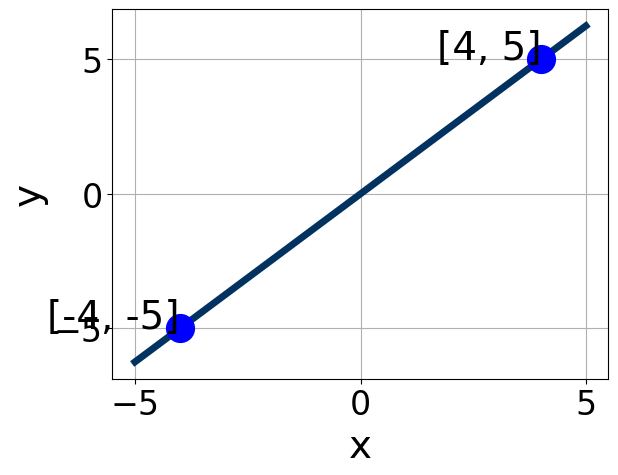
\includegraphics[width=0.5\textwidth]{../Figures/linearGraphToStandardC.png}
\end{center}
\begin{enumerate}[label=\Alph*.]
\item \( A \in [2.5, 6.6], \hspace{3mm} B \in [3.92, 5.01], \text{ and } \hspace{3mm} C \in [0, 2] \)
\item \( A \in [2.5, 6.6], \hspace{3mm} B \in [-4.36, -2.62], \text{ and } \hspace{3mm} C \in [0, 2] \)
\item \( A \in [-2.1, 0.6], \hspace{3mm} B \in [0.45, 2.18], \text{ and } \hspace{3mm} C \in [0, 2] \)
\item \( A \in [-5.8, -3.5], \hspace{3mm} B \in [3.92, 5.01], \text{ and } \hspace{3mm} C \in [0, 2] \)
\item \( A \in [-2.1, 0.6], \hspace{3mm} B \in [-2.37, -0.85], \text{ and } \hspace{3mm} C \in [0, 2] \)

\end{enumerate} }
\litem{
Solve the equation below. Then, choose the interval that contains the solution.\[ -7(18x + 11) = -14(6x + 5) \]\begin{enumerate}[label=\Alph*.]
\item \( x \in [3.35, 3.78] \)
\item \( x \in [-0.42, 0.59] \)
\item \( x \in [-3.78, -3.48] \)
\item \( x \in [-0.83, -0.38] \)
\item \( \text{There are no real solutions.} \)

\end{enumerate} }
\litem{
Solve the equation below. Then, choose the interval that contains the solution.\[ -19(-12x + 16) = -7(2x + 15) \]\begin{enumerate}[label=\Alph*.]
\item \( x \in [1.73, 2.49] \)
\item \( x \in [-1.95, -1.6] \)
\item \( x \in [0.24, 1.44] \)
\item \( x \in [1.37, 1.7] \)
\item \( \text{There are no real solutions.} \)

\end{enumerate} }
\litem{
Find the equation of the line described below. Write the linear equation as $ y=mx+b $ and choose the intervals that contain $m$ and $b$.\[ \text{Perpendicular to } 7 x + 3 y = 7 \text{ and passing through the point } (-6, -5). \]\begin{enumerate}[label=\Alph*.]
\item \( m \in [2.11, 2.89] \hspace*{3mm} b \in [-4.5, -0.1] \)
\item \( m \in [0.3, 0.47] \hspace*{3mm} b \in [-0.1, 1.9] \)
\item \( m \in [-0.76, -0.31] \hspace*{3mm} b \in [-8.2, -5.3] \)
\item \( m \in [0.3, 0.47] \hspace*{3mm} b \in [-4.5, -0.1] \)
\item \( m \in [0.3, 0.47] \hspace*{3mm} b \in [1.7, 5.1] \)

\end{enumerate} }
\litem{
First, find the equation of the line containing the two points below. Then, write the equation as $ y=mx+b $ and choose the intervals that contain $m$ and $b$.\[ (-3, 6) \text{ and } (11, -8) \]\begin{enumerate}[label=\Alph*.]
\item \( m \in [0.68, 1.32] \hspace*{3mm} b \in [-19, -18] \)
\item \( m \in [-1.02, -0.87] \hspace*{3mm} b \in [-3, -2] \)
\item \( m \in [-1.02, -0.87] \hspace*{3mm} b \in [1, 4] \)
\item \( m \in [-1.02, -0.87] \hspace*{3mm} b \in [-19, -18] \)
\item \( m \in [-1.02, -0.87] \hspace*{3mm} b \in [4, 11] \)

\end{enumerate} }
\litem{
Find the equation of the line described below. Write the linear equation as $ y=mx+b $ and choose the intervals that contain $m$ and $b$.\[ \text{Perpendicular to } 3 x - 7 y = 10 \text{ and passing through the point } (-5, -5). \]\begin{enumerate}[label=\Alph*.]
\item \( m \in [-1.3, 2] \hspace*{3mm} b \in [-17.67, -10.67] \)
\item \( m \in [-3.6, -1] \hspace*{3mm} b \in [-17.67, -10.67] \)
\item \( m \in [-3.6, -1] \hspace*{3mm} b \in [-1, 5] \)
\item \( m \in [-3.6, -1] \hspace*{3mm} b \in [15.67, 21.67] \)
\item \( m \in [1, 2.6] \hspace*{3mm} b \in [2.67, 8.67] \)

\end{enumerate} }
\litem{
Solve the linear equation below. Then, choose the interval that contains the solution.\[ \frac{3x -3}{7} - \frac{8x -4}{5} = \frac{-7x + 6}{4} \]\begin{enumerate}[label=\Alph*.]
\item \( x \in [2.2, 6.4] \)
\item \( x \in [1.5, 2.4] \)
\item \( x \in [7.7, 8.8] \)
\item \( x \in [-1.2, 1.9] \)
\item \( \text{There are no real solutions.} \)

\end{enumerate} }
\litem{
Solve the linear equation below. Then, choose the interval that contains the solution.\[ \frac{-3x -5}{8} - \frac{5x -6}{5} = \frac{-9x -4}{7} \]\begin{enumerate}[label=\Alph*.]
\item \( x \in [12.84, 16.84] \)
\item \( x \in [-16.04, -12.04] \)
\item \( x \in [52, 57] \)
\item \( x \in [-5.15, 1.85] \)
\item \( \text{There are no real solutions.} \)

\end{enumerate} }
\litem{
Write the equation of the line in the graph below in Standard form $Ax+By=C$. Then, choose the intervals that contain $A, B, \text{ and } C$.
\begin{center}
    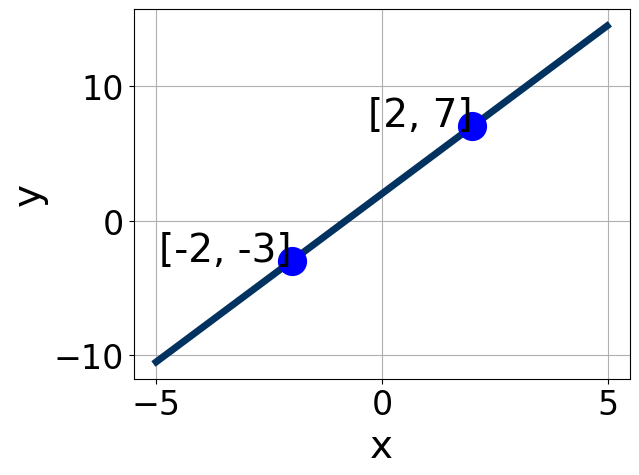
\includegraphics[width=0.5\textwidth]{../Figures/linearGraphToStandardCopyC.png}
\end{center}
\begin{enumerate}[label=\Alph*.]
\item \( A \in [-2.5, 1.5], \hspace{3mm} B \in [-0.39, 1.08], \text{ and } \hspace{3mm} C \in [-1, 2.3] \)
\item \( A \in [-2.5, 1.5], \hspace{3mm} B \in [-1.45, 0.59], \text{ and } \hspace{3mm} C \in [-2.5, -1.3] \)
\item \( A \in [1, 11], \hspace{3mm} B \in [1.79, 2.56], \text{ and } \hspace{3mm} C \in [2.3, 5.7] \)
\item \( A \in [1, 11], \hspace{3mm} B \in [-4.38, -1.89], \text{ and } \hspace{3mm} C \in [-6.8, -3.2] \)
\item \( A \in [-5, -3], \hspace{3mm} B \in [1.79, 2.56], \text{ and } \hspace{3mm} C \in [2.3, 5.7] \)

\end{enumerate} }
\end{enumerate}

\end{document}